\chapter{Análise do Sistema}

Este capítulo apresenta a análise da solução proposta para o Sebo do Cesar, descrevendo as funcionalidades esperadas, os atores envolvidos, os conceitos do domínio do problema e os requisitos que deverão ser atendidos pelo sistema. O objetivo é estabelecer uma visão estruturada da aplicação antes da definição dos aspectos de implementação e arquitetura técnica.

\section{Visão Geral do Sistema}
O sistema proposto consiste em uma aplicação web desenvolvida para apoiar a gestão operacional do Sebo do Cesar, centralizando informações relacionadas ao acervo de livros, estoque, clientes e vendas. A solução busca substituir ou reduzir controles manuais, fornecendo recursos para catalogação de livros, acompanhamento da disponibilidade de exemplares, registro de clientes, realização de vendas e geração de relatórios gerenciais. 
Além disso, o sistema prevê funcionalidades de recomendação de livros com base no histórico de compras dos clientes, contribuindo para a melhoria da experiência de atendimento. A plataforma será acessada por meio de navegadores web e disponibiliza uma interface simples e intuitiva, adequada ao contexto operacional do estabelecimento.

\section{Atores Envolvidos}
\begin{table}[htb]
\centering
\caption[Atores]{Atores.}
\label{tab-atores}
\begin{tabular}{p{2.6cm}|p{6.0cm}|p{2.25cm}|p{3.40cm}}
  %\hline
   \textbf{Ator} & \textbf{Descrição} \\
    \hline
    \textbf{Cliente} & Pessoa que frequenta a loja \\
    \hline
    \textbf{Funcionario} & Profissional que realizas as operações no local \\
    \hline
    \textbf{Gerente} & Acompanha métricas e relatórios \\
   % \hline
\end{tabular}
\end{table}

\section{Casos de Uso}
\begin{figure}[H]
	\caption{\label{fig_uso-cal}Casos de uso - Acervo}
	\begin{center}
	    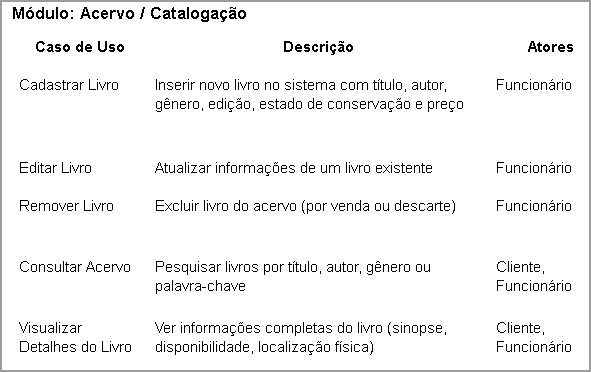
\includegraphics[scale=0.7]{imagens/uso_catal.png}
	\end{center}
\end{figure}

\begin{figure}[H]
	\caption{\label{fig_uso-client}Casos de uso - Cliente}
	\begin{center}
	    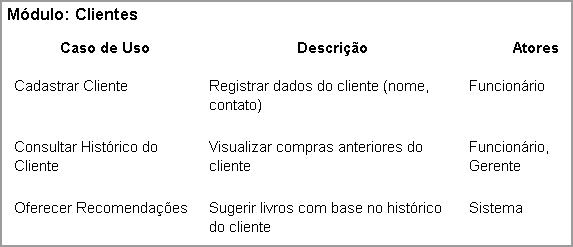
\includegraphics[scale=0.7]{imagens/uso_client.png}
	\end{center}
\end{figure}

\begin{figure}[H]
	\caption{\label{fig_uso-est}Casos de uso - Estoque}
	\begin{center}
	    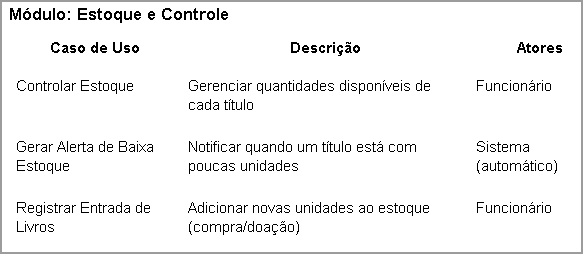
\includegraphics[scale=0.7]{imagens/uso_est.png}
	\end{center}
\end{figure}

\begin{figure}[H]
	\caption{\label{fig_uso-hist}Casos de uso - Histórico}
	\begin{center}
	    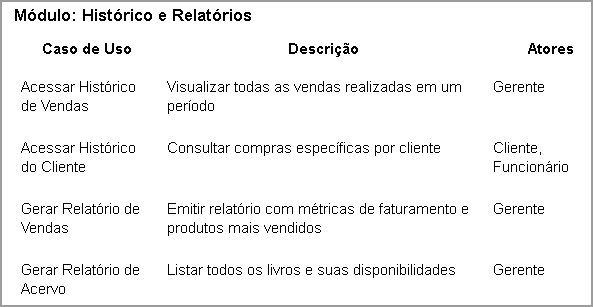
\includegraphics[scale=0.7]{imagens/uso_hist.png}
	\end{center}
\end{figure}

\begin{figure}[H]
	\caption{\label{fig_uso-vendas}Casos de uso - Vendas}
	\begin{center}
	    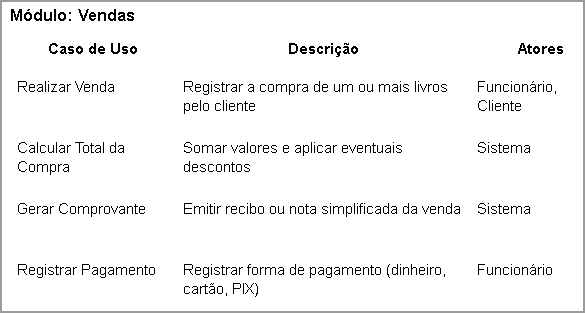
\includegraphics[scale=0.7]{imagens/uso_vendas.png}
	\end{center}
\end{figure}

\begin{figure}[H]
	\caption{\label{fig_rel-uso}Relacionamento Entre os Casos}
	\begin{center}
	    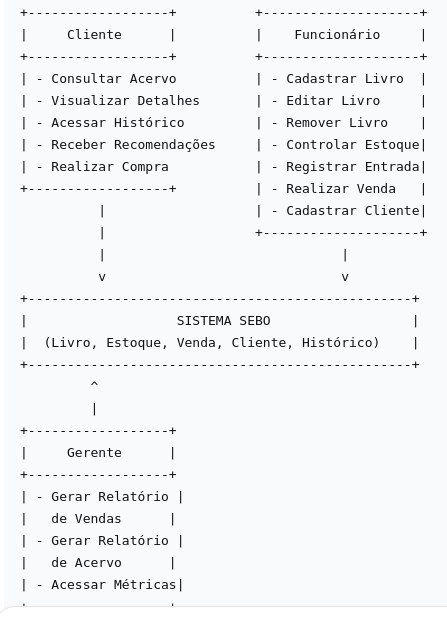
\includegraphics[scale=0.7]{imagens/rel_casos.png}
	\end{center}
\end{figure}

\section{Modelo Conceitual}
\begin{figure}[H]
	\caption{\label{fig_conc}Diagrama de Classes Conceitual}
	\begin{center}
	    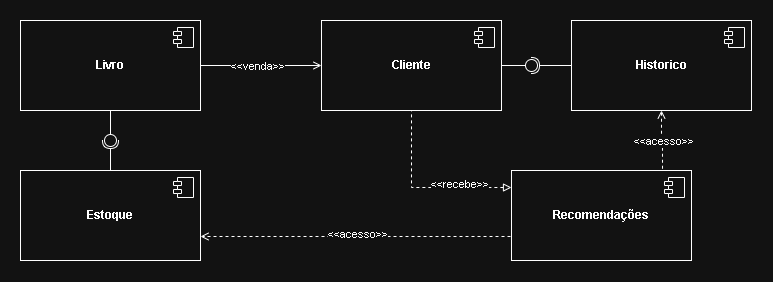
\includegraphics[scale=0.6]{imagens/diag_conc.png}
	\end{center}
\end{figure}

\section{Requisitos Funcionais}
\begin{figure}[H]
	\caption{\label{fig_rf-client}Requisitos Funcionais - Cliente}
	\begin{center}
	    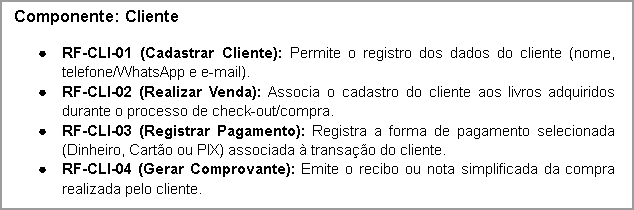
\includegraphics[scale=0.7]{imagens/rf_client.png}
	\end{center}
\end{figure}

\begin{figure}[H]
	\caption{\label{fig_rf-est}Requisitos Funcionais - Estoque}
	\begin{center}
	    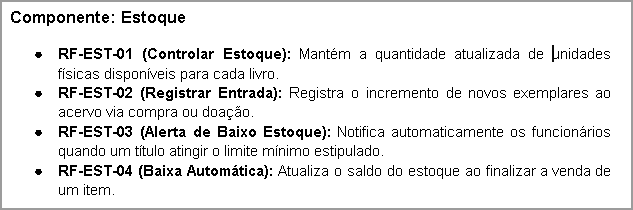
\includegraphics[scale=0.7]{imagens/rf_estoque.png}
	\end{center}
\end{figure}

\begin{figure}[H]
	\caption{\label{fig_rf-hist}Requisitos Funcionais - Histórico}
	\begin{center}
	    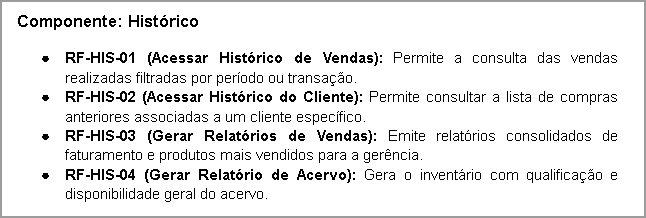
\includegraphics[scale=0.7]{imagens/rf_hist.png}
	\end{center}
\end{figure}

\begin{figure}[H]
	\caption{\label{fig_rf-livro}Requisitos Funcionais - Livro}
	\begin{center}
	    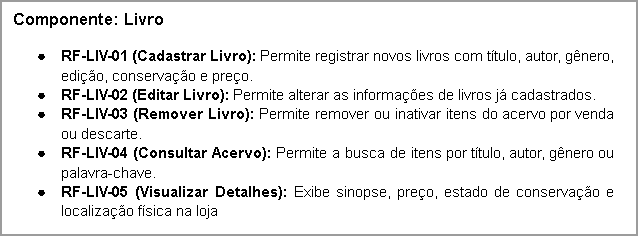
\includegraphics[scale=0.7]{imagens/rf_livro.png}
	\end{center}
\end{figure}

\begin{figure}[H]
	\caption{\label{fig_rf-recom}Requisitos Funcionais - Recomendação}
	\begin{center}
	    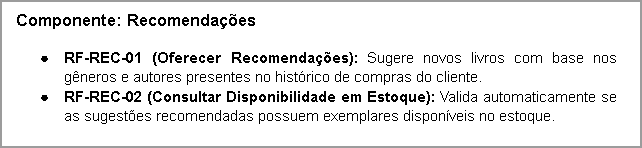
\includegraphics[scale=0.7]{imagens/rf_recom.png}
	\end{center}
\end{figure}

\section{Requisitos Não Funcionais}
\begin{figure}[H]
	\caption{\label{fig_nf-client}Requisitos Não Funcionais - Cliente}
	\begin{center}
	    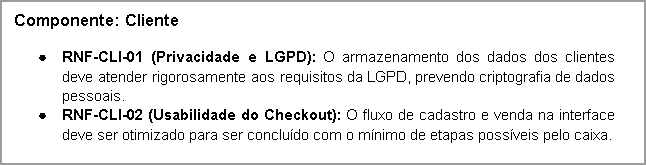
\includegraphics[scale=0.7]{imagens/nf_client.png}
	\end{center}
\end{figure}

\begin{figure}[H]
	\caption{\label{fig_nf-hist}Requisitos Não Funcionais - Histórico}
	\begin{center}
	    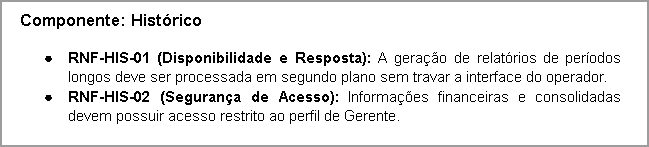
\includegraphics[scale=0.7]{imagens/nf_hist.png}
	\end{center}
\end{figure}

\begin{figure}[H]
	\caption{\label{fig_nf-est}Requisitos Não Funcionais - Estoque}
	\begin{center}
	    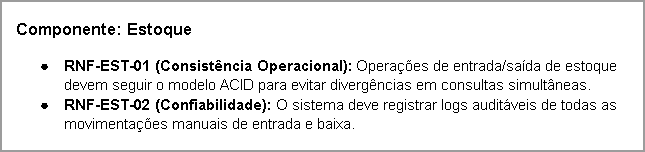
\includegraphics[scale=0.7]{imagens/nf_est.png}
	\end{center}
\end{figure}

\begin{figure}[H]
	\caption{\label{fig_nf-livro}Requisitos Não Funcionais - Livro}
	\begin{center}
	    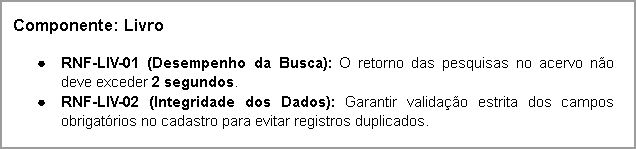
\includegraphics[scale=0.7]{imagens/nf_livro.png}
	\end{center}
\end{figure}

\begin{figure}[H]
	\caption{\label{fig_nf-recom}Requisitos Não Funcionais - Recomendação}
	\begin{center}
	    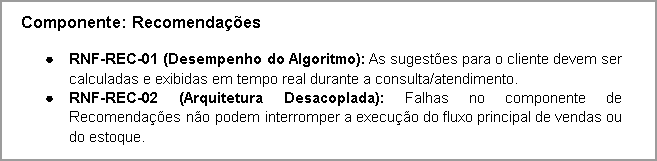
\includegraphics[scale=0.7]{imagens/nf_recom.png}
	\end{center}
\end{figure}

\section{Restrições do Sistema}
O desenvolvimento e a operação do sistema estão sujeitos a limitações legais e normativas que delimitam o escopo técnico do projeto. Dentre elas, destaca-se a conformidade com a LGPD \cite{brasil2018lgpd}, exigindo que a arquitetura da aplicação incorpore mecanismos robustos para o tratamento, armazenamento seguro e proteção de informações pessoais e sensíveis.
Do ponto de vista técnico e operacional, o projeto impõe restrições arquiteturais específicas. A comunicação entre a interface do usuário e o servidor deve seguir o padrão REST, garantindo o desacoplamento e a interoperabilidade dos componentes. Adicionalmente, a aplicação deve assegurar compatibilidade e responsividade com os principais navegadores web, operando sob protocolos de segurança de transporte baseados em criptografia (HTTPS/TLS) para salvaguardar a integridade e o sigilo das informações trafegadas na rede.